\documentclass{article}
\usepackage[utf8]{inputenc}
\usepackage{amsmath}
\usepackage{xcolor}
\usepackage[top=2cm, bottom=2cm, left=2cm, right=2cm]{geometry}
\setlength\parindent{0pt}

\usepackage{listings}
%\usepackage{color}
\usepackage{graphicx}
\usepackage{float}
\usepackage{caption}

\usepackage{verbatim}
\let\oldv\verbatim
\let\oldendv\endverbatim

%\userpackage{minted}

\definecolor{dkgreen}{rgb}{0,0.6,0}
\definecolor{gray}{rgb}{0.5,0.5,0.5}
\definecolor{mauve}{rgb}{0.58,0,0.82}
\definecolor{light-gray}{gray}{0.95}


\lstset{frame=tb,
  language=Java,
  aboveskip=6mm,
  belowskip=6mm,
  showstringspaces=false,
  columns=flexible,
  basicstyle={\small\ttfamily},
  numbers=none,
  numberstyle=\tiny\color{gray},
  keywordstyle=\color{blue},
  commentstyle=\color{dkgreen},
  stringstyle=\color{mauve},
  breaklines=true,
  breakatwhitespace=true,
  tabsize=3,
  backgroundcolor=\color{light-gray},
  language=Matlab
}

%\usepackage{natbib} replaced by line below to make refernces work
\usepackage[square,sort,comma,numbers]{natbib}
\usepackage[nottoc,numbib]{tocbibind} %to get references in table of contants
\usepackage{graphicx}

\usepackage{bm}

\usepackage{hyperref}
\hypersetup{
	colorlinks,
	citecolor=black,
	filecolor=black,
	linkcolor=black,
	urlcolor=black
}

\usepackage{mdframed}
\usepackage{lipsum} % for creating dummy text
\mdfdefinestyle{MyFrame}{%
	linecolor=black,	
	backgroundcolor=gray!20!white,
	skipbelow = 8mm,
	skipabove = 8mm}

\usepackage{scrextend}

\usepackage{multimedia}
\usepackage{media9}

\usepackage{booktabs}
\usepackage{adjustbox}

\title{Fys4150\\Project 5\\ }
\author{Peter Killingstad and Karl Jacobsen\\
\\
\url{https://github.com/kaaja/fys4150}}

\begin{document}
	
\maketitle

\section*{Note to instructurs reagarding Github repository}
If the above Github-link does not work, it is eighter because you have not yet accepted our invite to the repository, or you have not yet provided us with an e-mail addres available at Github so that we can invite you. The Github user you will be invited from is "kaaja". If the latter applies to you, please send us an e-mail with an e-mailadress available in Github or your Github username so that we can send you an invite. Our e-mailadresses: peter.killingstad@hotmail.com, karljaco@gmail.com.

\section{5a}

\subsection{Derivation of schemes with truncation errors}
All the schemes will be derived from Taylor series expansions, and the truncation error will be related to the remainder in the Taylor-series expansions. This remainded is the error we get when truncating the series by leaving out the remainder.\\

\subsection{Forward Euler}
For the time derivative, we expand $u(x, t + \Delta t)$ around $t$

\begin{subequations}
	\begin{align}
		u(x, t+ \Delta t)  = u(x,t) +  u_t(x,t) \Delta t + \mathcal{O}(\Delta t^2)\\
		\rightarrow u_t(x,t) = \frac{u(x, t+ \Delta t) - u(x,t)}{\Delta t} + \mathcal{O}(\Delta t)\label{eq:FeTime}
	\end{align}
\end{subequations}

The space derivative, which is a 2nd derivative, we derive by combining two Taylor series'

\begin{subequations}
	\begin{align}
		u(x + \Delta x,t) = u(x,t) + u_x(x,t)\Delta x + \frac{u_{xx}(x,t) \Delta x^2}{2} + \frac{u_{xxx}(x,t) \Delta x^3}{6} + \mathcal{O}(\Delta x^4)\label{eq:feSpace1}\\
		u(x - \Delta x,t) = u(x,t) - u_x(x,t)\Delta x + \frac{u_{xx}(x,t) \Delta x^2}{2} - \frac{u_{xxx}(x,t) \Delta x^3}{6} + \mathcal{O}(\Delta x^4)\label{eq:feSpace2}
	\end{align}
\end{subequations}

Now we add (\ref{eq:feSpace1}) and (\ref{eq:feSpace2}) and solve for $u_{xx}(x,t)$

\begin{subequations}
	\begin{align}
		\begin{split}
			\Big(u(x + \Delta x,t) + u(x - \Delta x,t) \Big) &= \Big(u(x,t) + u(x,t) \Big)\\ 
			&+ \Big(u_x(x,t)\Delta x + (- u_x(x,t)\Delta x) \Big)\\ 
			&+ \Big(\frac{u_{xx}(x,t) \Delta x^2}{2} +  \frac{u_{xx}(x,t) \Delta x^2}{2}\Big)\\ 
			&+ \Big(\frac{u_{xxx}(x,t) \Delta x^3}{6}  + (- \frac{u_{xxx}(x,t) \Delta x^3}{6}) \Big)\\ 
			&+ \Big(\mathcal{O}(\Delta x^4) + \mathcal{O}(\Delta x^4) \Big)
		\end{split}\\
		&= 2u(x,t) + u_{xx}(x,t) \Delta x^2 + \mathcal{O}(\Delta x^4)\\
		\rightarrow u_{xx}(x,t) &= \frac{u(x - \Delta x, t) - 2u(x,t) + u(x+ \Delta x, t)}{\Delta x^2} + \mathcal{O}(\Delta x^2)\label{eq:feSpace3}
	\end{align}
\end{subequations}

Combining (\ref{eq:FeTime}) and (\ref{eq:feSpace3}) we get the Forward Euler scheme

\begin{subequations}
	\begin{align}
		u_t(x,t) &= u_{xx}(x,t)\\
		\frac{u(x, t+ \Delta t) - u(x,t)}{\Delta t} + \mathcal{O}(\Delta t) &= 
		\frac{u(x - \Delta x, t) - 2u(x,t) + u(x+ \Delta x, t)}{\Delta x^2} + \mathcal{O}(\Delta x^2)\label{eq:fe}
	\end{align}
\end{subequations}

From (\ref{eq:fe}) we see that the scheme has a truncation error that goes like $\mathcal{O} (\Delta t)$ in time and $\mathcal{O}(\Delta x^2)$ in space.\\

We will now analyze the stability of the Forward Euler scheme (\ref{eq:fe}) by applying Neuman stability analyzis. From the analytical solution of the problem, we know that the particular solutions are on the form $u = e^{-(k \pi)^2 t}e^{i k \pi x}$, where $k$ is an integer greater than one. We observe that the solutions are stable in $t$, meaning that the solutions do not blow up as $t$ increaes. Based on the analytical particular solution, we make the numerical ansatz 

\begin{equation}\label{eq:neumanAnsatz}
	u = a_k^n e^{i k \pi x_j}
\end{equation}

For the numerical ansatz (\ref{eq:neumanAnsatz}) to reproduce the characteristics of the analytical particular solution, with stability in $t$, we observe that $|a_k^n| < 1$ in necessary. We now plug in the ansatz (\ref{eq:neumanAnsatz}) into the (\ref{eq:fe}) and derive an equation for $|a_k^n|$:

\begin{subequations}\label{eq:naumanFe0}
	\begin{align}
		\frac{u(x, t+ \Delta t) - u(x,t)}{\Delta t}  &= 
		\frac{u(x - \Delta x, t) - 2u(x,t) + u(x+ \Delta x, t)}{\Delta x^2} \\
		\frac{a_k^{n+1} e^{i k \pi (j+1) \Delta x} - a_k^n e^{i k \pi j \Delta x}}{\Delta t}  &= 
		\frac{a_k^{n} e^{i k \pi (j-1) \Delta x} - 2a_k^{n} e^{i k \pi j \Delta x} + a_k^{n} e^{i k \pi (j+1) \Delta x}}{\Delta x^2} \\
		a_k^{n} e^{i k \pi j \Delta x}\; \frac{a_k  -1}{\Delta t}  &= 
		a_k^{n} e^{i k \pi j \Delta x}\; \frac{ e^{-i k \pi \Delta x} - 2  +  e^{i k \pi  \Delta x}}{\Delta x^2} \\
		 \frac{a_k  -1}{\Delta t}  &= 
		 \frac{ e^{-i k \pi \Delta x} - 2  +  e^{i k \pi  \Delta x}}{\Delta x^2} \\
		 a_k &= 1 + \frac{\Delta t}{\Delta x^2} (e^{-i k \pi \Delta x} - 2  +  e^{i k \pi  \Delta x})\\
		 &= 1+ \frac{\Delta t}{\Delta x^2} \Big(2 \cos(k\pi\Delta x) - 2\Big)\\
		 &= 1+ 2\frac{\Delta t}{\Delta x^2} \Big( \cos(k\pi\Delta x) - 1\Big)\\
		 &= 1+ 2\frac{\Delta t}{\Delta x^2} \Big(- 2 \sin^2(\frac{k\pi\Delta x}{2}) \Big)\\
		 &=1 - 4\frac{\Delta t}{\Delta x^2} \sin^2(\frac{k\pi\Delta x}{2}) \\
		 |a_k| &= |1 - 4\frac{\Delta t}{\Delta x^2} \sin^2(\frac{k\pi\Delta x}{2})|\label{eq:neumanFe1}
	\end{align}
\end{subequations}

From (\ref{eq:neumanFe1}) we get
 
\begin{subequations}
	\begin{align}
		 &|a_k| < 1\; \text{if}\; ||1 - 4\frac{\Delta t}{\Delta x^2} \sin^2(\frac{k\pi\Delta x}{2})|| < 1 \\
		 &\rightarrow |1 - 4 \frac{\Delta t}{\Delta x^2}| < 1 \rightarrow |a_k| < 1\;\text{(Since $\sin^2(k \pi \Delta x/2)_{max}  = 1$)}\\
		 &\rightarrow 1 - 4 \frac{\Delta t}{\Delta x^2} > -1\\ 
		 &\rightarrow \frac{\Delta t}{\Delta x^2} < \frac{1}{2}\label{eq:neumanFe2}
	\end{align}
\end{subequations}

(\ref{eq:neumanFe2}) gives that the Forward Euler scheme is conditionally stable, and the condition that ensures stability.


\subsection{Backward Euler}
Here we will do the same as we did for Forward Euler above: Derive the scheme, including truncation errors, and analyze stability.\\

The only change compared to Forward Euler, is the time discretization, which now becomes

\begin{subequations}
	\begin{align}
	u(x, t- \Delta t)  = u(x,t) +  u_t(x,t) \Delta t - \mathcal{O}(\Delta t^2)\\
	\rightarrow u_t(x,t) = \frac{u(x, t) - u(x,t - \Delta t)}{\Delta t} + \mathcal{O}(\Delta t)\label{eq:beTime}
	\end{align}
\end{subequations}

The space discretization is the same as for Forward Euler, (\ref{eq:feSpace3}). Combining the space discretization (\ref{eq:feSpace3}) and (\ref{eq:beTime}) gives

\begin{subequations}
	\begin{align}
		\frac{u(x, t) - u(x,t - \Delta t)}{\Delta t} + \mathcal{O}(\Delta t) = \frac{u(x - \Delta x, t) - 2u(x,t) + u(x+ \Delta x, t)}{\Delta x^2} + \mathcal{O}(\Delta x^2)\label{eq:be1}
	\end{align}
\end{subequations}

We note that the truncation errors have the same asymptoptic behavior as for the Forward Euler scheme. \\

Now lets check the stability of the Backward Euler scheme. We apply the same method as we did for Forward Euler, and insert the ansatz (\ref{eq:neumanAnsatz}) into (\ref{eq:be1}) to get

\begin{subequations}
	\begin{align}
		\frac{u(x, t) - u(x,t - \Delta t)}{\Delta t}  &= \frac{u(x - \Delta x, t) - 2u(x,t) + u(x+ \Delta x, t)}{\Delta x^2} \\
		\frac{a_k^n e^{i k \pi j \Delta x} - a_k^{n-1} e^{i k \pi j \Delta x}}{\Delta t}  &= \frac{a_k^n e^{i k \pi (j -1)\Delta x} - 2a_k^n e^{i k \pi j \Delta x} + a_k^n e^{i k \pi (1 + j)\Delta x}}{\Delta x^2} \\
		a_k^n e^{i k \pi j \Delta x}\; \frac{1 - a_k^{-1}}{\Delta t}&=
		a_k^n e^{i k \pi j \Delta x}\; \frac{e^{-i k \pi \Delta x} - 2 + e^{i k \pi \Delta x}}{\Delta x^2}\\
		\frac{1 - a_k^{-1}}{\Delta t}&= \frac{e^{-i k \pi \Delta x} - 2 + e^{i k \pi \Delta x}}{\Delta x^2}\\
		a_k^{-1} &= 1 - \frac{\Delta t}{\Delta x^2} (e^{-i k \pi \Delta x} - 2 + e^{i k \pi \Delta x})\\
		a_k &= \frac{1}{1 - \frac{\Delta t}{\Delta x^2} (e^{-i k \pi \Delta x} - 2 + e^{i k \pi \Delta x})}\\
		&\stackrel{(\ref{eq:naumanFe0})}{=}  \frac{1}{1 + 4 \frac{\Delta t}{\Delta x^2} \sin^2(\frac{k\pi\Delta x}{2})}\\
		|a_k| &=  \left|\frac{1}{1 + 4 \frac{\Delta t}{\Delta x^2} \sin^2(\frac{k\pi\Delta x}{2})}\right| < 1.\label{eq:neumanBe}\\
	\end{align}
\end{subequations}

From (\ref{eq:neumanBe}) we see that, in contrast to the Forward Euler scheme, the Backward Euler scheme is unconditionally stable.\\


(\ref{eq:be1}) reveals another difference between the Backward Euler scheme and the Forward Euler scheme: (\ref{eq:be1}) is implicit in $u(x,t)$, meaning that we cannot solve (\ref{eq:be1}) directly for $u(x,t)$, as we did in the Forward Euler scheme. However, we can find $u(x,t)$ from (\ref{eq:be1}) by recognizing that (\ref{eq:be1}) can be rewritten as a linear system:

\begin{subequations}
	\begin{align}
		\frac{u(x, t) - u(x,t - \Delta t)}{\Delta t}  &= \frac{u(x - \Delta x, t) - 2u(x,t) + u(x+ \Delta x, t)}{\Delta x^2} \\
		\frac{u_i^n - u_i^{n-1}}{\Delta t}  &= \frac{u_{i-1}^n - 2u_i^n + u_{i+1}^n}{\Delta x^2} \\
		\frac{\Delta x^2}{\Delta t}(u_i^n - u_i^{n-1})  &=  u_{i-1}^n - 2u_i^n + u_{i+1}^n\\
		- \Big(u_{i-1}^n - (2 + \frac{\Delta x^2}{\Delta t}) u_i^n + u_{i+1}^n\Big)   &=  \frac{\Delta x^2}{\Delta t}u_i^{n-1}\\
		 \Big(-u_{i-1}^n + (2 + \frac{\Delta x^2}{\Delta t}) u_i^n - u_{i+1}^n\Big)   &=  \frac{\Delta x^2}{\Delta t}u_i^{n-1}\\
		\underbrace{\begin{bmatrix} 2 + \frac{\Delta x^2}{\Delta t} & -1 & \cdots & 0 \\ -1 & 2 + \frac{\Delta x^2}{\Delta t} & -1 & \vdots \\
			\vdots & &  \ddots & \vdots \\ 
			0 & \cdots & -1 & 2 + \frac{\Delta x^2}{\Delta t} \end{bmatrix}}_{\mathbf{A}} 
		\underbrace{\begin{bmatrix} u_1^n\\ u_2^n \\ \vdots\\ u_N^n \end{bmatrix}}_{\mathbf{U}} &= 
		\underbrace{\frac{\Delta x^2}{\Delta t} \begin{bmatrix} u_0^{n-1}\\ u_1^{n-1} \\ \vdots \\ u_N^{n-1}\end{bmatrix}}_{\mathbf{\tilde{b}}}\label{eq:beLinSys}
	\end{align}
\end{subequations}

We see from (\ref{eq:beLinSys}) that solving Backward Euler corresponds to solving a linear system $A U = \tilde{b}$, where $A$ is a trdiagonal matrix. 
	
\subsection{Crank-Nicolson}
Here we Taylor expand $u(x+\Delta x, t+\Delta t)$ and $u(x-\Delta x, t+\Delta t)$ around $t'=t+\Delta t/2$ to get

\begin{subequations}
	\begin{align}
		\begin{split}
			u(x+\Delta x, t+\Delta t)&=u(x,t')+\frac{\partial u(x,t')}{\partial x}\Delta x+\frac{\partial u(x,t')}{\partial t} \frac{\Delta t}{2} +\frac{\partial^2 u(x,t')}{2\partial x^2}\Delta x^2+\frac{\partial^2 u(x,t')}{2\partial t^2}\frac{\Delta t^2}{4}\\ 
			&+\frac{\partial^2 u(x,t')}{\partial x\partial t}\frac{\Delta t}{2} \Delta x+ \mathcal{O}(\Delta t^3)
		\end{split}\label{eq:cn1}\\
		\begin{split}
			u(x-\Delta x,t+ \Delta t)&=u(x,t')
			-\frac{\partial u(x,t')}{\partial x}\Delta x 
			+ \frac{\partial u(x,t')}{\partial t} \frac{\Delta t}{2} +\frac{\partial^2 u(x,t')}{2\partial x^2}\Delta x^2
			+\frac{\partial^2 u(x,t')}{2\partial t^2}\frac{\Delta t^2}{4}\\ 
			&- \frac{\partial^2 u(x,t')}{\partial x\partial t}\frac{\Delta t}{2} \Delta x
			+ \mathcal{O}(\Delta t^3)
		\end{split}\label{eq:cn2}\\
		\begin{split}
			u(x+\Delta x,t)&=u(x,t')+\frac{\partial u(x,t')}{\partial x}\Delta x-\frac{\partial u(x,t')}{\partial t} \frac{\Delta t}{2} +\frac{\partial^2 u(x,t')}{2\partial x^2}\Delta x^2+\frac{\partial^2 u(x,t')}{2\partial t^2}\frac{\Delta t^2}{4} \\
			&- \frac{\partial^2 u(x,t')}{\partial x\partial t}\frac{\Delta t}{2} \Delta x+ \mathcal{O}(\Delta t^3)
		\end{split}\label{eq:cn3}\\
		\begin{split}
		u(x-\Delta x,t)&=u(x,t')-\frac{\partial u(x,t')}{\partial x}\Delta x-\frac{\partial u(x,t')}{\partial t} \frac{\Delta t}{2} +\frac{\partial^2 u(x,t')}{2\partial x^2}\Delta x^2+\frac{\partial^2 u(x,t')}{2\partial t^2}\frac{\Delta t^2}{4}\\
		& +\frac{\partial^2 u(x,t')}{\partial x\partial t}\frac{\Delta t}{2} \Delta x+ \mathcal{O}(\Delta t^3)
		\end{split}\label{eq:cn4}\\
		u(x,t+\Delta t)&=u(x,t')+\frac{\partial u(x,t')}{\partial t}\frac{\Delta_t}{2} +\frac{\partial ^2 u(x,t')}{2\partial t^2}\Delta t^2 + \mathcal{O}(\Delta t^3)\label{eq:cn5}\\
		u(x,t)&=u(x,t')-\frac{\partial u(x,t')}{\partial t}\frac{\Delta t}{2}+\frac{\partial ^2 u(x,t')}{2\partial t^2}\Delta t^2 + \mathcal{O}(\Delta t^3)\label{eq:cn6}
	\end{align}
\end{subequations}

The above formulae are taken from Hjorth-Jensen's  \href{https://github.com/CompPhysics/ComputationalPhysics/tree/master/doc/pub/pde}{slides} \cite{MHJ2}.\\

Combining (\ref{eq:cn5}) and (\ref{eq:cn6}) gives the time derivative

\begin{subequations}
	\begin{align}
		\begin{split}
			\Big(u(x,t+\Delta t) - u(x,t)\Big) &= \Big(u(x,t') -  u(x,t')\Big) + \Big(\frac{\partial u(x,t')}{\partial t}\frac{\Delta_t}{2} - (-\frac{\partial u(x,t')}{\partial t}\frac{\Delta t}{2}) \Big)\\ 
			&+ \Big(\frac{\partial ^2 u(x,t')}{2\partial t^2}\Delta t^2 - \frac{\partial ^2 u(x,t')}{2\partial t^2}\Delta t^2 \Big) +\Big(\mathcal{O}(\Delta t^3) -  \mathcal{O}(\Delta t^3)\Big)
		\end{split}\\
		u(x,t+\Delta t) - u(x,t)& = \frac{\partial u(x,t')}{\partial t}\Delta t + \mathcal{O}(\Delta t^3)\\
		\frac{\partial u(x,t')}{\partial t}&= \frac{u(x,t+\Delta t) - u(x,t)}{\Delta t} + \mathcal{O}(\Delta t^2)\label{eq:cnTime}
	\end{align}
\end{subequations}

Now for the spacial derivative. First we solve (\ref{eq:cn1}) and (\ref{eq:cn2}) for $u_{xx}(x, t')$

\begin{subequations}
	\begin{align}
		\begin{split}
		u(x+\Delta x, t+\Delta t) + u(x-\Delta x,t + \Delta t) &= 
		\Big(u(x,t') + u(x,t') \Big) + \Big(\frac{\partial u(x,t')}{\partial x}\Delta x-\frac{\partial u(x,t')}{\partial x}\Delta x\Big)\\ 
		&+ \Big(\frac{\partial u(x,t')}{\partial t} \frac{\Delta t}{2} +\frac{\partial u(x,t')}{\partial t} \frac{\Delta t}{2} \Big) + \Big(\frac{\partial^2 u(x,t')}{2\partial x^2}\Delta x^2+\frac{\partial^2 u(x,t')}{2\partial x^2}\Delta x^2\Big)\\
		& + \Big(\frac{\partial^2 u(x,t')}{2\partial t^2}\frac{\Delta t^2}{4} +\frac{\partial^2 u(x,t')}{2\partial t^2}\frac{\Delta t^2}{4} \Big) + \Big(\frac{\partial^2 u(x,t')}{\partial x\partial t}\frac{\Delta t}{2} \Delta x - \frac{\partial^2 u(x,t')}{\partial x\partial t}\frac{\Delta t}{2} \Delta x\Big)\\
		& + \Big(\mathcal{O}(\Delta t^3) + \mathcal{O}(\Delta t^3) \Big) + \mathcal{O}(\Delta x^4)
		\end{split}\\
		\begin{split}
			&=2u(x,t') + \frac{\partial u(x,t')}{\partial t} \Delta t
			+ \frac{\partial^2 u(x,t')}{\partial x^2}\Delta x^2
			 + \frac{\partial^2 u(x,t')}{2\partial t^2}\frac{\Delta t^2}{2}  
			 + \mathcal{O}(\Delta t^3) + \mathcal{O}(\Delta x^4)
		\end{split}\\
		\begin{split}
			&=2u(x,t') + \frac{\partial u(x,t')}{\partial t} \Delta t
			+ \frac{\partial^2 u(x,t')}{\partial x^2}\Delta x^2			
			+ \mathcal{O}(\Delta t^2) + \mathcal{O}(\Delta x^4)
		\end{split}\\	
		\begin{split}
		\frac{\partial^2 u(x,t')}{\partial x^2}\Delta x^2
		& = 
		u(x+\Delta x, t+\Delta t) + u(x-\Delta x,t + \Delta t) 
		- 2u(x,t') 
			\\ 
		&+\frac{\partial u(x,t')}{\partial t} \Delta t
		+  \mathcal{O}(\Delta t^2) + \mathcal{O}(\Delta x^4)
		\end{split}\\
		\begin{split}
			\frac{\partial^2 u(x,t')}{\partial x^2}
			&=\frac{u(x-\Delta x,t+ \Delta t)  - 2u(x,t') +  	u(x+\Delta x, t+\Delta t)}{\Delta x^2}\\
			& +\frac{\partial u(x,t')}{\partial t} \frac{\Delta t}{\Delta x^2} +\mathcal{O}(\Delta t^2) + \mathcal{O}(\Delta x^2)\label{eq:cnX2}
		\end{split}		
	\end{align}
\end{subequations}

Note that in (\ref{eq:cnX2}) we added $\mathcal{O}(\Delta x^4)$, since  $\mathcal{O}(\Delta x^3)$ cancells out in the addition. Also note that the $\Delta x^3$-term was not originally  included in (\ref{eq:cn1}) and  (\ref{eq:cn2}), but these would have been of equal magnitude with opposite sign, so when adding the equaions we would have been left with $\mathcal{O}(\Delta x^4)$.\\

Doing the same as in (\ref{eq:cnX2}) for (\ref{eq:cn3}) and (\ref{eq:cn4}) we obtain

\begin{subequations}\label{eq:cnX3}
	\begin{align}
		\begin{split}
			\frac{\partial^2 u(x,t')}{\partial x^2} &=\frac{u(x-\Delta x,t) - 2u(x,t') + u(x+\Delta x, t)}{\Delta x^2}\\
			&- \frac{\partial u(x,t')}{\partial t} \frac{\Delta t}{\Delta x^2} 
			+  \mathcal{O}(\Delta t^2) + \mathcal{O}(\Delta x^2)
		\end{split}
	\end{align}
\end{subequations}

Now we take the mean of (\ref{eq:cnX2}) and (\ref{eq:cnX3}) 

\begin{subequations}
	\begin{align}
		\begin{split}
			u_{xx}(x, t^{'}) &=\frac{1}{2} \Big(\frac{u(x-\Delta x,t+ \Delta t)  - 2u(x,t') +  	u(x+\Delta x, t+\Delta t)}{\Delta x^2} +\frac{\partial u(x,t')}{\partial t} \frac{\Delta t}{\Delta x^2} + \mathcal{O}(\Delta t^2) + \mathcal{O}(\Delta x^2) \\
			&+  \frac{u(x-\Delta x,t) - 2u(x,t') + u(x+\Delta x, t)}{\Delta x^2} -\frac{\partial u(x,t')}{\partial t} \frac{\Delta t}{\Delta x^2} + \mathcal{O}(\Delta t^2)  + \mathcal{O}(\Delta x^2)\Big)\\
			&= \frac{1}{2} \Big(\frac{u(x-\Delta x,t+ \Delta t)  - 2u(x,t') +  	u(x+\Delta x, t+\Delta t)}{\Delta x^2} \\
			& +  \frac{u(x-\Delta x,t) - 2u(x,t') + u(x+\Delta x, t)}{\Delta x^2} \Big) + \mathcal{O}(\Delta t^2) + \mathcal{O}(\Delta x^2)\\
			&\stackrel{u(x,t^{'}) = \frac{u(x,t) + u(x,t+\Delta t)}{2}}{=}\\
			&\frac{1}{2} \Big(\frac{u(x-\Delta x,t+ \Delta t)  - u(x,t) + u(x,t+\Delta t) +  	u(x+\Delta x, t+\Delta t)}{\Delta x^2} \\
			& +  \frac{u(x-\Delta x,t) - u(x,t) + u(x,t+\Delta t) + u(x+\Delta x, t)}{\Delta x^2} \Big) + \mathcal{O}(\Delta t^2) + \mathcal{O}(\Delta x^2)\\
			&= \frac{1}{2} \Big(\frac{u(x-\Delta x,t+ \Delta t) - 2u(x,t+\Delta t) +u(x + \Delta x,t+\Delta t)}{\Delta x^2} + \frac{u(x-\Delta x,t) - 2u(x,t) +u(x+ \Delta x,t)}{\Delta x^2} \Big)\\
			& + \mathcal{O}(\Delta t^2)  + \mathcal{O}(\Delta x^2)\label{eq:cnX4}
			\end{split}
	\end{align}
\end{subequations}

Now combining (\ref{eq:cnTime}) and (\ref{eq:cnX4}) we get the Crank-Nicolson scheme

\begin{subequations}\label{eq:cn1d}
	\begin{align}
		\begin{split}
			\frac{u(x,t+\Delta t) - u(x,t)}{\Delta t} + \mathcal{O}(\Delta t^2)
			&= \frac{1}{2} \Big(\frac{u(x-\Delta x,t+ \Delta t)
			- 2u(x,t+\Delta t) +u(x+\Delta x,t+\Delta t)}{\Delta x^2} \\
			&+ \frac{u(x-\Delta x,t) - 2u(x,t) +u(x+ \Delta x,t)}{\Delta x^2} \Big) + \mathcal{O}(\Delta x^2),
		\end{split}
	\end{align}
\end{subequations}

where we have put both $\mathcal{O}(\Delta t^2)$ into a common term.\\

(\ref{eq:cn1d}) shows that the Crank-Nicolson scheme is 2nd order in both time and space, implying better convergence properties for the Crank-Nicolson scheme compared to the Backward Euler scheme and the Forward Euler scheme.\\

Using the same method as we used for the previous schemes, we  now study the stability of the Crank-Nicolson scheme. We insert the ansatz (\ref{eq:neumanAnsatz}) into the Crank-Nicolson scheme (\ref{eq:cn1d}) and solve for $|a_k|$:

\begin{subequations}
	\begin{align}
		\begin{split}
			\frac{u(x,t+\Delta t) - u(x,t)}{\Delta t} 
			&= \frac{1}{2} \Big(\frac{u(x-\Delta x,t+ \Delta t)
			- 2u(x,t+\Delta t) +u(x+\Delta x,t+\Delta t)}{\Delta x^2} \\
			&+ \frac{u(x-\Delta x,t) - 2u(x,t) +u(x+ \Delta x,t)}{\Delta x^2} \Big) \\
			a_k^n e^{i k \pi j \Delta x}\; \frac{ a_k  - 1}{\Delta t} &= \frac{a_k^n e^{i k \pi j \Delta x}}{2}\; \Big(\frac{a_k e^{-i k \pi \Delta x} - 2a_k + a_k e^{i k \pi \Delta x}}{\Delta x^2} + \frac{e^{-i k \pi \Delta x} - 2 +  e^{i k \pi \Delta x}}{\Delta x^2} \Big)\\
			\frac{ a_k  - 1}{\Delta t}&=\frac{1}{2}\Big(\frac{a_k e^{-i k \pi \Delta x} - 2a_k + a_k e^{i k \pi \Delta x}}{\Delta x^2} + \frac{e^{-i k \pi \Delta x} - 2 +  e^{i k \pi \Delta x}}{\Delta x^2} \Big)\\
			&= \frac{1+a_k}{2\Delta x^2} (e^{-i k \pi \Delta x} - 2 + e^{i k \pi \Delta x})\\
			&\stackrel{(\ref{eq:naumanFe0})}{=} -4\frac{1+a_k}{2\Delta x^2} \sin^2(\frac{k\pi \Delta x}{2})\\
			a_k -1 &= (1 + a_k) (-\frac{2 \Delta t}{\Delta x^2})\sin^2(\frac{k\pi \Delta x}{2})\\
			\Big(1 +\frac{2 \Delta t}{\Delta x^2}\sin^2(\frac{k\pi \Delta x}{2})\Big)a_k &= 1 - \frac{2 \Delta t}{\Delta x^2}\sin^2(\frac{k\pi \Delta x}{2})
			\end{split}\\
			a_k &= \frac{1 - \frac{2 \Delta t}{\Delta x^2}\sin^2(\frac{k\pi \Delta x}{2})}{1 +\frac{2 \Delta t}{\Delta x^2}\sin^2(\frac{k\pi \Delta x}{2})} < 1\label{eq:neumanCn1d}
	\end{align}
\end{subequations}

(\ref{eq:neumanCn1d}) shows that the Crank-Nicolson scheme is unconditionally stable.\\

Based on the analyzis of the different schemes, we expect the Crank-Nicolson scheme to be the best scheme with respect to convergence and stability. 

\subsection{$\theta$-rule}
All the schemes derived above can be derived from a more general scheme, called the $\theta$-rule scheme. To see this, first notice that the Crank-Nicolson scheme (\ref{eq:cn1d}) is the average of the Forward Euler scheme (\ref{eq:fe}) and the Backward Euler scheme (\ref{eq:be1}). We can think of the average, represented by the Crank-Nicolson scheme, as the special case of equals weights in a weighted average of the Backward Euler scheme and the Forward Euler scheme. Writing the weighted average of the Forward Euler and Backward Euler schemes with weights $0 \leq \theta \leq1$, we get the $\theta$-rule

\begin{subequations}
	\begin{align}
		\begin{split}
			(1-\theta) 	\frac{u(x,t+\Delta t) - u(x,t)}{\Delta t} + \theta 	\frac{u(x,t+\Delta t) - u(x,t)}{\Delta t}&=  \theta \frac{u(x-\Delta x,t+ \Delta t)
				- 2u(x,t+\Delta t) +u(x+\Delta x,t+\Delta t)}{\Delta x^2} \\
			&+ (1 - \theta) \frac{u(x-\Delta x,t) - 2u(x,t) +u(x+ \Delta x,t)}{\Delta x^2} 
		\end{split}\\
		\begin{split}
			\frac{u(x,t+\Delta t) - u(x,t)}{\Delta t}&= 
			  \theta \frac{u(x-\Delta x,t+ \Delta t)
				- 2u(x,t+\Delta t) +u(x+\Delta x,t+\Delta t)}{\Delta x^2} \\
			&+ (1 - \theta) \frac{u(x-\Delta x,t) - 2u(x,t) +u(x+ \Delta x,t)}{\Delta x^2} 
			\end{split}\label{eq:thetaRule}
	\end{align}
\end{subequations}

From the $\theta$-scheme (\ref{eq:thetaRule}) we see that $\theta = 0,\;1/2,\;1$ corresponds to the Forward Euler, the Crank-Nicolson and the Backward Euler scheme respectively.\\

When implementing the 1D-schemes, we will use the $\theta$-scheme. Using the $\theta$-scheme, we need only write one scheme instead of three.

\subsection{Implementation of 1D problem}
As mentioned in the previous paragraph, we implement the 1D schemes using the $\theta$-scheme. We will now rewrite (\ref{eq:thetaRule}) to a linear system, and then we will apply the Thomas algorithm to this system.\\

To ease the notation, we introduce 

\begin{equation}\label{eq:alpha}
	\alpha = \frac{\Delta t}{\Delta x^2}.
\end{equation}

Insertion of $\alpha$ (\ref{eq:alpha}) into the $\theta$-scheme (\ref{eq:thetaRule}) and introdusing the discretization $u(x + \Delta x, t - \Delta t) = u_{i+1}^{n-1}$ gives

\begin{subequations}
	\begin{align}
		\begin{split}
				&\frac{u(x,t+\Delta t) - u(x,t)}{\Delta t}= 
		\theta \frac{u(x-\Delta x,t+ \Delta t)
			- 2u(x,t+\Delta t) +u(x+\Delta x,t+\Delta t)}{\Delta x^2} \\
		&+ (1 - \theta) \frac{u(x-\Delta x,t) - 2u(x,t) +u(x+ \Delta x,t)}{\Delta x^2} 
		\end{split}\\
		\begin{split}
			&u(x,t+\Delta t) - u(x,t)= 
			\alpha \theta \Big(u(x-\Delta x,t+ \Delta t)
				- 2u(x,t+\Delta t) +u(x+\Delta x,t+\Delta t)\Big) \\
			&+ \alpha (1 - \theta) \Big(u(x-\Delta x,t) - 2u(x,t) +u(x+ \Delta x,t)\Big) 
		\end{split}\\
			&u_i^{n+1} - u_i^{n}= 
			\alpha \theta \Big(u_{i-1}^{n+1}
			- 2u_i^{n+1} +u_{i+1}^{n+1}\Big) + \alpha (1 - \theta) \Big(u_{i-1}^n - 2u_i^n +u_{i+1}^n\Big) \\
		&u_i^{n} - u_i^{n-1}= 
		\alpha \theta \Big(u_{i-1}^{n}
		- 2u_i^{n} +u_{i+1}^{n}\Big) + \alpha (1 - \theta) \Big(u_{i-1}^{n-1} - 2u_i^{n-1} +u_{i+1}^{n-1}\Big) \\
			&u_i^{n} -\alpha \theta \Big(u_{i-1}^{n}
			- 2u_i^{n} +u_{i+1}^{n}\Big) = u_i^{n-1} 
			 + \alpha (1 - \theta) \Big(u_{i-1}^{n-1} - 2u_i^{n-1} +u_{i+1}^{n-1}\Big)\\
			&-\alpha \theta u_{i-1}^{n} +
			(2 \alpha \theta + 1) u_i^{n} - \alpha \theta u_{i+1}^{n} = 
			 \alpha (1 - \theta) u_{i-1}^{n-1} +\Big(1 - 2 \alpha (1 - \theta) \Big)u_i^{n-1} +\alpha (1 - \theta)u_{i+1}^{n-1}\\
			 &-2\alpha \theta u_{i-1}^{n} +
			 2(2 \alpha \theta + 1) u_i^{n} - 2\alpha \theta u_{i+1}^{n} = 
			 2\alpha (1 - \theta) u_{i-1}^{n-1} +2\Big(1 - 2 \alpha (1 - \theta) \Big)u_i^{n-1} +2\alpha (1 - \theta)u_{i+1}^{n-1}\label{eq:thetaAlgo1}
	\end{align}
\end{subequations}

Now we rewrite (\ref{eq:thetaAlgo1}) as a matrix-vector equation $A_1 U^n = A_2 U^{n-1}$:

\begin{subequations}
	\begin{align}
		\begin{split}
		\underbrace{\begin{bmatrix} 2(2 \alpha \theta + 1) & - 2\alpha \theta & \cdots & 0 \\ - 2\alpha \theta & 2(2 \alpha \theta + 1) & - 2\alpha \theta & \vdots \\
			\vdots & &  \ddots & - 2\alpha \theta \\ 
			0 & \cdots & - 2\alpha \theta &2(2 \alpha \theta + 1) \end{bmatrix}}_{\mathbf{A_1}} 
		\underbrace{\begin{bmatrix} u_1^n\\ u_2^n \\ \vdots\\ u_N^n \end{bmatrix}}_{\mathbf{U^{n}}}\\ = 
		\underbrace{\begin{bmatrix} 2( 1 - 2 \alpha (1-\theta)) &  2\alpha (1-\theta) & \cdots & 0 \\  2\alpha (1-\theta) & 2( 1 - 2 \alpha (1-\theta)) &  2\alpha (1-\theta) & \vdots \\
	\vdots & &  \ddots &  2\alpha (1-\theta) \\ 
	0 & \cdots &  2\alpha (1-\theta) &2( 1 - 2 \alpha (1-\theta)) \end{bmatrix}}_{\mathbf{A_2}} 
	\underbrace{\begin{bmatrix} u_1^{n-1}\\ u_2^{n-1} \\ \vdots\\ u_N^{n-1} \end{bmatrix}}_{\mathbf{U^{n-1}}}	
		\end{split}\label{eq:thetaLinsSys}
	\end{align}
\end{subequations}

In (\ref{eq:thetaLinsSys}), the right hand side $\mathbf{A_2 U^{n-1}}$ is known, since $\mathbf{U}^{n-1}$ is the previous periods solution, so (\ref{eq:thetaLinsSys}) is a linear system of the known type $A U = b$. So in principle the above system is solved for each time step, solving it for a time step and then using this solution in the right hand side in the next time step.\\

We note that with $\theta = 0$ in (\ref{eq:thetaLinsSys}), the system reduces to the explicit Forward Euler system, which can be obtained from (\ref{eq:fe}). $\theta  = 1$ gives the Backward Euler system (\ref{eq:beLinSys}). $\theta = 1/2$ in (\ref{eq:thetaLinsSys}) gives the system that can be obtained by rewrting the Crank-Nicolson scheme (\ref{eq:cn1d}) as a linear system.\\

In principle the above system can be solved by calculating the inverse of $A_1$ and solving $U^n = A_1^{-1} (A_2 U^{n-1})$. This is a costly operation and is avoided. Instead of calculating the inverse, one often solves these systems by some kind of elimination method, e.g. Gaussian elimination or by LU. In this case, we note that we are dealing with a tridiagonal matrix. For tridiagonal systems, the Thomas algorithm gives an alterative way of solving the linear system which reduces the number of FLOPS considerably. In our case we are eaven more lucky. Our matrix is symmetric, and the elements are constant, so the standard Thomas algorithm can be further improved. We will now derive the algorithm that we implement.\\

We start with a tridiagonal symmetric linear system $Au =f$, with $A$ being $4 \times 4$. The following show the forward substitution steps for this sytem

\begin{subequations}
	\begin{align}
		\begin{bmatrix}
		     d_1 & e_1 & 0 & 0 & f_1\\
		      e_2 & d_2 & e_2 & 0 & f_2\\
			 0 & e_3 & d_3 & e_3 & f_3\\
	         0 & 0 & e_4 & d_4 & f_4
		\end{bmatrix}
		\rightarrow
		\begin{bmatrix}
		d_1 & e_1 & 0 & 0 & f_1\\
		0 & \tilde{d}_2 & e_2 & 0 & \tilde{f}_2\\
		0 & e_3 & d_3 & e_3 & f_3\\
		0 & 0 & e_4 & d_4 & f_4
		\end{bmatrix}
		\rightarrow
		\begin{bmatrix}
		d_1 & e_1 & 0 & 0 & f_1\\
		0 & \tilde{d}_2 & e_2 & 0 &\tilde{f}_2 \\
		0 & 0 & \tilde{d}_3 & e_3 & \tilde{f}_3\\
		0 & 0 & e_4 & d_4 & f_4
		\end{bmatrix}
		\rightarrow
		\begin{bmatrix}
		d_1 & e_1 & 0 & 0 & f_1\\
		0 & \tilde{d}_2 & e_2 & 0 &\tilde{f}_2 \\
		0 & 0 & \tilde{d}_3 & e_3 & \tilde{f}_3\\
		0 & 0 & e_4 & \tilde{d}_4 & \tilde{f}_4
		\end{bmatrix}
	\end{align}\label{eq:thomas1}
\end{subequations}


From (\ref{eq:thetaLinsSys}) we have that in our case $e_1=e_2 = ... = e_N= -2 \alpha$ and $d_1 = d_2 = ... = d_N = 2(2\alpha \theta +1)$. Calculating the first couple of $\tilde{d}$'s we quickly see that we get the following general expression for $\tilde{d}_i$

\begin{equation}\label{eq:thomasDtilde}
	\tilde{d}_i = 2(2\alpha \theta +1) + \frac{(2\alpha)^2}{\tilde{d}_{i-1}}\;\text{for } i>1.
\end{equation}

Doing the same for $\tilde{f}$ we get the general expression

\begin{equation}\label{eq:thomasFtilde}
	\tilde{f}_i = f_i + \frac{2 \alpha \theta}{\tilde{d}_{i-1}} \tilde{f}_{i-1}\;\text{for } i>1.
\end{equation}

Having $\tilde{d}$ and $\tilde{f}$ we are ready to do the back substitution step. We have

\begin{subequations}
	\begin{align}
		\begin{bmatrix}
		d_1 & e_1 & 0 & 0\\
		0 & \tilde{d}_2 & e_2 & 0  \\
		0 & 0 & \tilde{d}_3 & e_3 \\
		0 & 0 & e_4 & \tilde{d}_4 
		\end{bmatrix}
		\begin{bmatrix} u_1\\ u_2 \\ u_3\\ u_4  \end{bmatrix}
		= \begin{bmatrix} f_1\\\tilde{f}_2 \\ \tilde{f}_3\\ \tilde{f}_4  \end{bmatrix}
	\end{align}\label{eq:thomasBack1}
\end{subequations}

From (\ref{eq:thomasBack1}) we get

\begin{equation}\label{eq:thomasULast}
	u_4 = \frac{\tilde{f}_4}{\tilde{d}_4}
\end{equation}

and

\begin{equation}\label{eq:thomasU}
	u_i = \frac{\tilde{f}_i + 2\alpha \theta u_{i+1}}{\tilde{d}_i}\; \text{for } i > 1.
\end{equation}

The equations (\ref{eq:thomasDtilde}), (\ref{eq:thomasFtilde}), (\ref{eq:thomasULast}) and (\ref{eq:thomasU}) is what we need for our algorithm.

\begin{lstlisting}
for time in times:
	Calculate RHS f (= A_2 U^{n-1})
	
	// Forward substitution
	for row in rows (Start from 1st row):
		Calculate \tilde{d}
		Calculate \tilde{f}
	end row loop
	
	// Backward substitution
	For row in rows (Starting from last row)
		Calculate u
	end row loop

	// Update RHS for next time step
	U^{n-1} = U^{n}

end time loop
\end{lstlisting}

\subsection{2D schemes}
We will derive and apply a Forward Euler (explicit) scheme and a Backward Euler (implicit) scheme for the 2D case.

\subsubsection{2D explicit scheme}
The new thing in the 2D case for the explicit scheme, is that we get an extra term for $u_{yy}$ in (\ref{eq:fe}). $u_{yy}$ is approximated in exactly the same way as $u_{xx}$ (\ref{eq:feSpace3}), so we get

\begin{equation}
	 u_{yy}(x,y,t) = \frac{u(x,y - \Delta y, t) - 2u(x,y,t) + u(x,y+ \Delta y, t)}{\Delta y^2} + \mathcal{O}(\Delta y^2)\label{eq:uyyFe2d}
\end{equation}

Adding (\ref{eq:uyyFe2d}) to the 1D FE scheme (\ref{eq:fe}) gives the explicit 2D-scheme

\begin{subequations}
	\begin{align}
		\begin{split}
			\frac{u(x,y, t+ \Delta t) - u(x,y,t)}{\Delta t} + \mathcal{O}(\Delta t) &= 
			\frac{u(x - \Delta x, y,t) - 2u(x,y,t) + u(x+ \Delta x,y, t)}{\Delta x^2} \\
			&+  \frac{u(x,y - \Delta y, t) - 2u(x,y,t) + u(x,y+ \Delta y, t)}{\Delta y^2} \\
			&+ \mathcal{O}(\Delta x^2)  + \mathcal{O}(\Delta y^2)
		\end{split}\\
		\rightarrow u_{ij}^{n+1} &\stackrel{(\ref{eq:alpha})}{\approx} u_{ij}^{n} + \alpha (u_{i-1,j}^n + u_{i+1,j}^n + u_{i,j-1}^n + u_{i,j+1}^n - 4u_{ij}^n),\label{eq:Fe2d}
	\end{align}
\end{subequations}

where we in the last transition assumed $\Delta x = \Delta y$ such that $\alpha$ is given as before.\\

First we observe that the truncation errors go like $\mathcal{O}(\Delta t)$, $\mathcal{O}(\Delta x^2)$ and $\mathcal{O}(\Delta y^2)$.\\

Now lets analyze the stability, by inserting the ansatz

\begin{equation}\label{eq:ansatz2d}
	u = a_k^n e^{i k \pi \Delta x j} e^{i k \pi \Delta y l}
\end{equation}

into (\ref{eq:Fe2d}) and solve for $|a|$, as before\\

\begin{subequations}
	\begin{align}
		u_{ij}^{n+1} &= u_{ij}^{n} + \alpha (u_{i-1,j}^n + u_{i+1,j}^n + u_{i,j-1}^n + u_{i,j+1}^n - 4u_{ij}^n)\\
		a_k^n e^{i \pi k \Delta x j} e^{i \pi k \Delta j l} a&= 
		a_k^n e^{i \pi k \Delta x j} e^{i \pi k \Delta j l} 
		\Big(1 + \alpha(e^{-i k \pi \Delta x} + e^{i k \pi \Delta x})  - 2 + e^{-i k \pi \Delta y} + e^{i k \pi \Delta y})  - 2\Big)\\
		a&= 
		\Big(1 + \alpha(e^{-i k \pi \Delta x} + e^{i k \pi \Delta x})  - 2 + e^{-i k \pi \Delta y} + e^{i k \pi \Delta y})  - 2\Big)\\
		&\stackrel{(\ref{eq:naumanFe0})}{=}
		1 - 4 \alpha \Big(\sin^2 (k \pi \Delta x /2) + \sin^2(k \pi \Delta y/2)\Big)\\
		|a| &=
		\left|1 - 4 \alpha \Big(\sin^2 (k \pi \Delta x /2) + \sin^2(k \pi \Delta y/2)\Big)\right|\\
		|a| < 1 &\rightarrow 		\left|1 - 4 \alpha \Big(\sin^2 (k \pi \Delta x /2) + \sin^2(k \pi \Delta y/2)\Big)\right|  < 1\label{eq:2dFeStab1}\\
		&\left|1 - 4 \alpha \Big(\sin^2 (k \pi \Delta x /2) + \sin^2(k \pi \Delta y/2)\Big)\right| < \left|1 - 8 \alpha \right|\label{eq:2dFeStab2}
	\end{align}
\end{subequations}

Again assuming $\Delta x = \Delta y$, we have $\alpha = \Delta t/\Delta x^2 > 0$, so that (\ref{eq:2dFeStab1}) and (\ref{eq:2dFeStab2}) gives

\begin{subequations}
	\begin{align}
		1 - 8 \alpha < -1\\
		\alpha < \frac{1}{4}.\label{eq:2dFeStab}
	\end{align}
\end{subequations}

(\ref{eq:2dFeStab}) gives that the 2D Forward Euler scheme is conditionally stable. We note that we could probably have applied a simpler ansatz than (\ref{eq:ansatz2d}), since it in (\ref{eq:Fe2d}) was already assumed that $\Delta x = \Delta y$. \\


The new thing in (\ref{eq:Fe2d}) compared to (\ref{eq:fe}), is that $u{ij}^{n+1}$ in the 2D case is a matrix and not a vector as in the 1D case. The fact that we are dealing with a matrix instead of a vector, does not change anything with regards to the solution strategy. The equation (\ref{eq:Fe2d}) is still explicit, the only difference in implementation is that instead of one single loop a double loop over two space dimensions is needed now.\\

The algorithm for solving 2D Forward Euler follows.

\begin{lstlisting}
Set IC

for time in times:
	Set BC
	
	for x in X:
		for y in Y:
			Calculate u_{ij}^{n+1} = f(u^{n})
		end y-loop
	end x-loop
	
	Set u^{n} = u^{n+1}	
	
end time-loop
\end{lstlisting}

\subsubsection{2D implicit scheme}
We start in the same way as we did for Forward Euler in 2D, and just add an extra term for $u_{yy}$ to the 1D Backward Euler scheme (\ref{eq:be1}). In addition we will assume $h = \Delta x = \Delta y$.

\begin{subequations}
	\begin{align}
		\begin{split}
			\frac{u(x,y, t) - u(x,y,t - \Delta t)}{\Delta t} + \mathcal{O}(\Delta t) &= \frac{u(x - \Delta x,y, t) 
				- 2u(x,y,t) + u(x+ \Delta x,y, t)}{\Delta x^2} \\
			&+ \frac{u(x,y - \Delta y, t) - 2u(x,y,t) + u(x,y+ \Delta y, t)}{\Delta y^2}\\
			&+ \mathcal{O}(\Delta x^2) + \mathcal{O}(\Delta y^2)
		\end{split}\\
		\begin{split}
		\frac{u_{i,j}^n - u_{i,j}^{n-1}}{\Delta t}  &\approx \frac{u_{i-1,j}^{n} 
			- 2u_{i,j}^n + u_{i+1,j}^n}{\Delta x^2} \\
		&+ \frac{u_{i,j-1}^n - 2u_{i,j}^n + u_{i,j+1}^n}{\Delta y^2}
		\end{split}\\
		\begin{split}
			\frac{u_{i,j}^n - u_{i,j}^{n-1}}{\Delta t} &\stackrel{h = \Delta x = \Delta y}{\approx} \frac{u_{i-1,j}^{n} 
			- 2u_{i,j}^n + u_{i+1,j}^n}{h^2} \\
			&+ \frac{u_{i,j-1}^n - 2u_{i,j}^n + u_{i,j+1}^n}{h^2}
		\end{split}\\				
		u_{i,j}^n - u_{i,j}^{n-1}  &\stackrel{(\ref{eq:alpha})}{\approx} \alpha (u_{i-1,j}^{n} 
			- 4u_{i,j}^n + u_{i+1,j}^n + u_{i,j-1}^n + u_{i,j+1}^n)\label{eq:2dBe1}\\
		u_{i,j}^n &= u_{i,j}^{n-1}  + \frac{1}{1+4\alpha}(u_{i-1,j}^{n} 
		+ u_{i+1,j}^n + u_{i,j-1}^n + u_{i,j+1}^n)\label{eq:2dBe}
	\end{align}
\end{subequations}

First we observe that the truncation errors go like $\mathcal{O}(\Delta t)$, $\mathcal{O}(\Delta x^2)$ and $\mathcal{O}(\Delta y^2)$, so there is no difference in the truncation errors between Forward Euler and Backward Euler, just as for the 1D case.\\

We study stability of the 2D Backward Euler scheme by inerting the 2D ansatz (\ref{eq:ansatz2d}) into
(\ref{eq:2dBe1})

\begin{subequations}
	\begin{align}
	u_{i,j}^n - u_{i,j}^{n-1} 
	&=
	\alpha (u_{i-1,j}^{n} 
	- 4u_{i,j}^n + u_{i+1,j}^n + u_{i,j-1}^n + u_{i,j+1}^n)\\
	a_k - 1 &= \alpha a (e^{-ik \pi \Delta x} + e^{ik \pi \Delta x} -2 + e^{-ik \pi \Delta y} + e^{ik \pi \Delta y} -2 )\\
	&\stackrel{(\ref{eq:naumanFe0})}{=} - 4 \alpha a \Big(\sin^2(k \pi \Delta x/2) +  \sin^2(k \pi \Delta y/2)\Big)\\
	&\stackrel{\Delta x = \Delta y = h}{=} -8 \alpha a \sin^2(kh/2)\\
	a &= \frac{1}{1+ 8 \alpha \sin^2(kh/2)} < 1\label{eq:2dBeStability}
	\end{align}
\end{subequations}

From (\ref{eq:2dBeStability}) we see that the Backward Euler scheme is also unconditionally stable in two dimensions, as it was for one dimension. We note that we probably could have applied a simpler ansatz than (\ref{eq:ansatz2d}), since it in (\ref{eq:2dBe1}) was already assumed that $\Delta x = \Delta y$.\\

We see that (\ref{eq:2dBe}) is an implicit scheme, since the only known is $u_{i,j}^n$. (\ref{eq:2dBe}) can be transformed into a linear system of the known type $Au = b$. The procedure for transforming (\ref{eq:2dBe}) into a linear system is the same as demonstrated for the 1D case, see Hjorth-Jensen \cite{MHJ} p. 317. However, there is one important difference compared to the 1D linear system: The matrix is not tridiagonal anymore! This means that we cannot apply the Thomas algorithm anymore, and standard methods as LU-decomposion becomes unpractical. However, in our case the matrix is positive definite, implying that iterative schemes converges to the tru solution, Hjorth-Jensen \cite{MHJ} p. 322. Iterative methods are often much faster than direct methods like Gaussian elimination and LU-decomposition. Hence we will solve the implicit problem applying iterative methods. 

\subsubsection{Iterative methods}
This section follows Olver and Shakiban's \cite{olver} chapter on iterative methods closesly. The goal is to present the main idea behind iterative methods, and to present the Jacobi method as part of a general framework.\\

Firstly, an iterative method is not a direct method, like e.g. Gaussian elemination, that solves the problem as it is stated, typically 

\begin{equation}\label{eq:AuB}
	\mathbf{A}\mathbf{u} = \mathbf{b}.
\end{equation} 

Instead, with iterative methods, one solves another problem:

\begin{equation}\label{eq:iter1}
	\mathbf{u}^{k+1} = \mathbf{T} \mathbf{u}^k + \mathbf{c},
\end{equation}
where $k$ stands for iterations. \\

For the iterative method to work, it firstly has to converge: 

\begin{equation}\label{eq:itConver}
	\lim_{k \rightarrow \infty} \mathbf{u}^{k} = \mathbf{u}^{*}.
\end{equation}

Taking the limit on both sides of (\ref{eq:iter1}) and using (\ref{eq:itConver}) we get

\begin{subequations}
	\begin{align}
			\lim_{k \rightarrow \infty} \mathbf{u}^{k+1} &= 	\lim_{k \rightarrow \infty} \mathbf{T} \mathbf{u}^k + \mathbf{c}\\
			\mathbf{u}^{*} &= \mathbf{T} \mathbf{u}^{*} + \mathbf{c}.\label{eq:itFixedPoint}
	\end{align}
\end{subequations}

(\ref{eq:itFixedPoint}) is a fixed point equation, and we have that the solution to the iterative scheme has to converge to a fixed point.\\
 
Secondly, the convergent solution $\mathbf{u}^{*}$ that is approached  as $k \rightarrow \infty$ must become equal to the solution $\mathbf{u}$ of the original problem, $\mathbf{A}\mathbf{u} = \mathbf{b}$. \\

Lets now look at conditions for the 1st condition, convergence to the fixed point $\mathbf{u^{*}}$ to hold. We study the error with respect to the fixed point

\begin{subequations}
	\begin{align}
		\mathbf{e}^{k+1} &= \mathbf{u}^{k+1} - \mathbf{u}^{*}\\
		&\stackrel{(\ref{eq:iter1})}{=}  \mathbf{T} \mathbf{u}^k + \mathbf{c} - \mathbf{u}^{*}\\
		&=\mathbf{T} \mathbf{u}^k + \mathbf{c} - (\mathbf{T} \mathbf{u}^{*} + \mathbf{c})\\
		&=\mathbf{T} (\mathbf{u}^k -\mathbf{u}^{*}\\
		&=\mathbf{T}\mathbf{e}^{k}\\
		&=\mathbf{T}^k\mathbf{e}^{(0)}.\label{eq:iterConvError}
	\end{align}
\end{subequations}

(\ref{eq:iterConvError}) shows that the development of the error in convergence towards the fixed point depends on the same matrix as the original iterative problem, $\mathbf{T}$. We have convergende towards the fixed point $\mathbf{u}^{*}$ if $\mathbf{T}$ is a convergent matrix. $\mathbf{T}$ is a convergent matrix if the spectral radius of $\mathbf{T}$ is less than one, $\rho(T) < 1$. The speed of convergence is inversly related to the spectral radius, implying that we want to construct $T$ with as low spectral radius as possible.  \\

We now have a condition for the first requirement for our iterative scheme: convergence to the fixed point. Now for the 2nd condition: convergence to the true solution. An iterative scheme converging to a fixed point different from the true solution is of little use in our case. It turns out that convergence to the true solution depeneds on the chosen scheme, represented by the matrix $T$ in our case, and the coefficient matrix of the original problem, $A$. We have that both the Jacobi scheme, to be derived, and the Gauss-Seidel scheme are convergent to the true solution if $A$ is strictly diagonally dominant.\\

We sum up our results in this section:\\

The iteration scheme (\ref{eq:iter1}) converges to the solution of the original linear system (\ref{eq:AuB}) if the following two conditions are satisfied

\begin{itemize}
	\item{The spectral radius of $T$ in (\ref{eq:iter1}) is less than one.}
	
	\item{$A$ in (\ref{eq:AuB}) is strictly diagonally dominant (In the case of Jacobi and Gauss-Seidel)}
\end{itemize}

Next we will derive the Jacobi-algorithm and relate it to our genereal iterative system (\ref{eq:iter1}).

\subsubsection{Jacobi's algorithm}
We begin by a rewrite of the linear system (\ref{eq:AuB}), where we split $A$ into one strictly lower triangular matrix, $L$, one strictly upper triangular matrix, $U$, and one diagonal matrix, $D$:

\begin{subequations}
	\begin{align}
		A \mathbf{u} &= \mathbf{b}\\
		(L + D + U) \mathbf{u} &= \mathbf{b}\\
		\mathbf{u} &= D^{-1} \Big(-(L+D) \mathbf{u} + \mathbf{b}\Big)\label{eq:iterJacobi1}
	\end{align}
\end{subequations}

The above is nothing new. It is still the original system. With the Jacobi algorithm, one sets $\mathbf{u}^{k+1} = \mathbf{u}$ on the left hand side of (\ref{eq:iterJacobi1}) and $\mathbf{u} = \mathbf{u}^k$ on the right hand side to get

\begin{subequations}
	\begin{align}
	\mathbf{u}^{k+1}  &= D^{-1} \Big(-(L+D) \mathbf{u}^k + \mathbf{b}\Big)\label{eq:iterJacobi2}
	\end{align}
\end{subequations}

We see that the Jacobi-scheme (\ref{eq:iterJacobi2}) fits our general iterative fixed point scheme (\ref{eq:iter1}), with

\begin{subequations}\label{eq:jacobiFixed}
	\begin{align}
		&T = -D^{-1}(L+D)\\
		&\mathbf{c} = D^{-1} \mathbf{b}.
	\end{align}
\end{subequations}

It is perhaps easier to see that the Jacbi algoritm (\ref{eq:iterJacobi2}) do by considering a single row in the matrix-vector system

\begin{subequations}\label{eq:jacobiRow}
	\begin{align}
		u_i^{(k+1)} = - \frac{1}{a_{ii}} \sum_{j=1,i \neq j} a_{ij} u_j^{(k)} + \frac{b_i}{a_{ii}}.
	\end{align}
\end{subequations}

Using (\ref{eq:jacobiRow}) we will in the next section see that it is easy to formulate a Jacobi-solver for the 2D implicit scheme (\ref{eq:2dBe}).

\subsubsection{Jacobi's algorithm applied to the 2D implicit diffusion}
Now we will apply Jacobi's algorithm (\ref{eq:jacobiRow}) to the 2D implicit scheme (\ref{eq:2dBe}). We see that (\ref{eq:2dBe}) is already almost set up like a Jacobi-scheme. We get

\begin{subequations}\label{eq:jacobi2D}
	\begin{align}
				u_{i,j}^{n,(k+1)} &= u_{i,j}^{n-1}  + \frac{1}{1+4\alpha}(u_{i-1,j}^{n, (k)} 
		+ u_{i+1,j}^{n,(k)} + u_{i,j-1}^{n,(k)} + u_{i,j+1}^{n,(k)})
	\end{align}
\end{subequations}

(\ref{eq:jacobi2D}) is our Jacobi-Solver. By setting

\begin{subequations}
	\begin{align}
		&a_{ii} = -(1 + 4\alpha)\\
		&b_i = a_{ii} u_{i,j}^{n-1}
	\end{align}
\end{subequations}

in (\ref{eq:jacobi2D}) we see that (\ref{eq:jacobi2D}) corresponds to the Jacobi-algorithm (\ref{eq:jacobiRow}). We also note that only 4 neighboring pints are needed.\\

Following Hjorth-Jensen \cite{MHJ} p. 319, we get the following main algorithm for the Jacobi-solver

\begin{itemize}
	\item{1: Make intial guess for $u_{i,j}$ for all internal points.}
	\item{2: Caclulate iteration $k$ of $u$, $u^k$ using (\ref{eq:2dBe})}.
	\item{3: Stop if wanted convergence reached, else continue next iteration.}
	\item{4: Set previous $u$-value equal to new $u$.}
	\item{5: Repeat all steps from step 2.}
\end{itemize}

The above algorithm is used for all time steps, starting with the first internal time step, solving one step at the time before moving to the next step.

\subsection{2D Physical problem with boundary conditions}
We choose to model a laminar flow inside an infinite tunnel with a finite quadratic cross section. We only model a single cross section, the problem being identical for all cross sections because of the homogenity assumption in the flow direction. \\

There will be no slip boundary conditions on all four walls. The floor and the sides will be fixed, while the roof will be moving in the flow direction. With these boundary conditions we have zero velocity on the floor and the side walls, while we have a non-zero velcocity in the flow direction. The figure below shows our problem.

\begin{figure}[H]
	\centering
	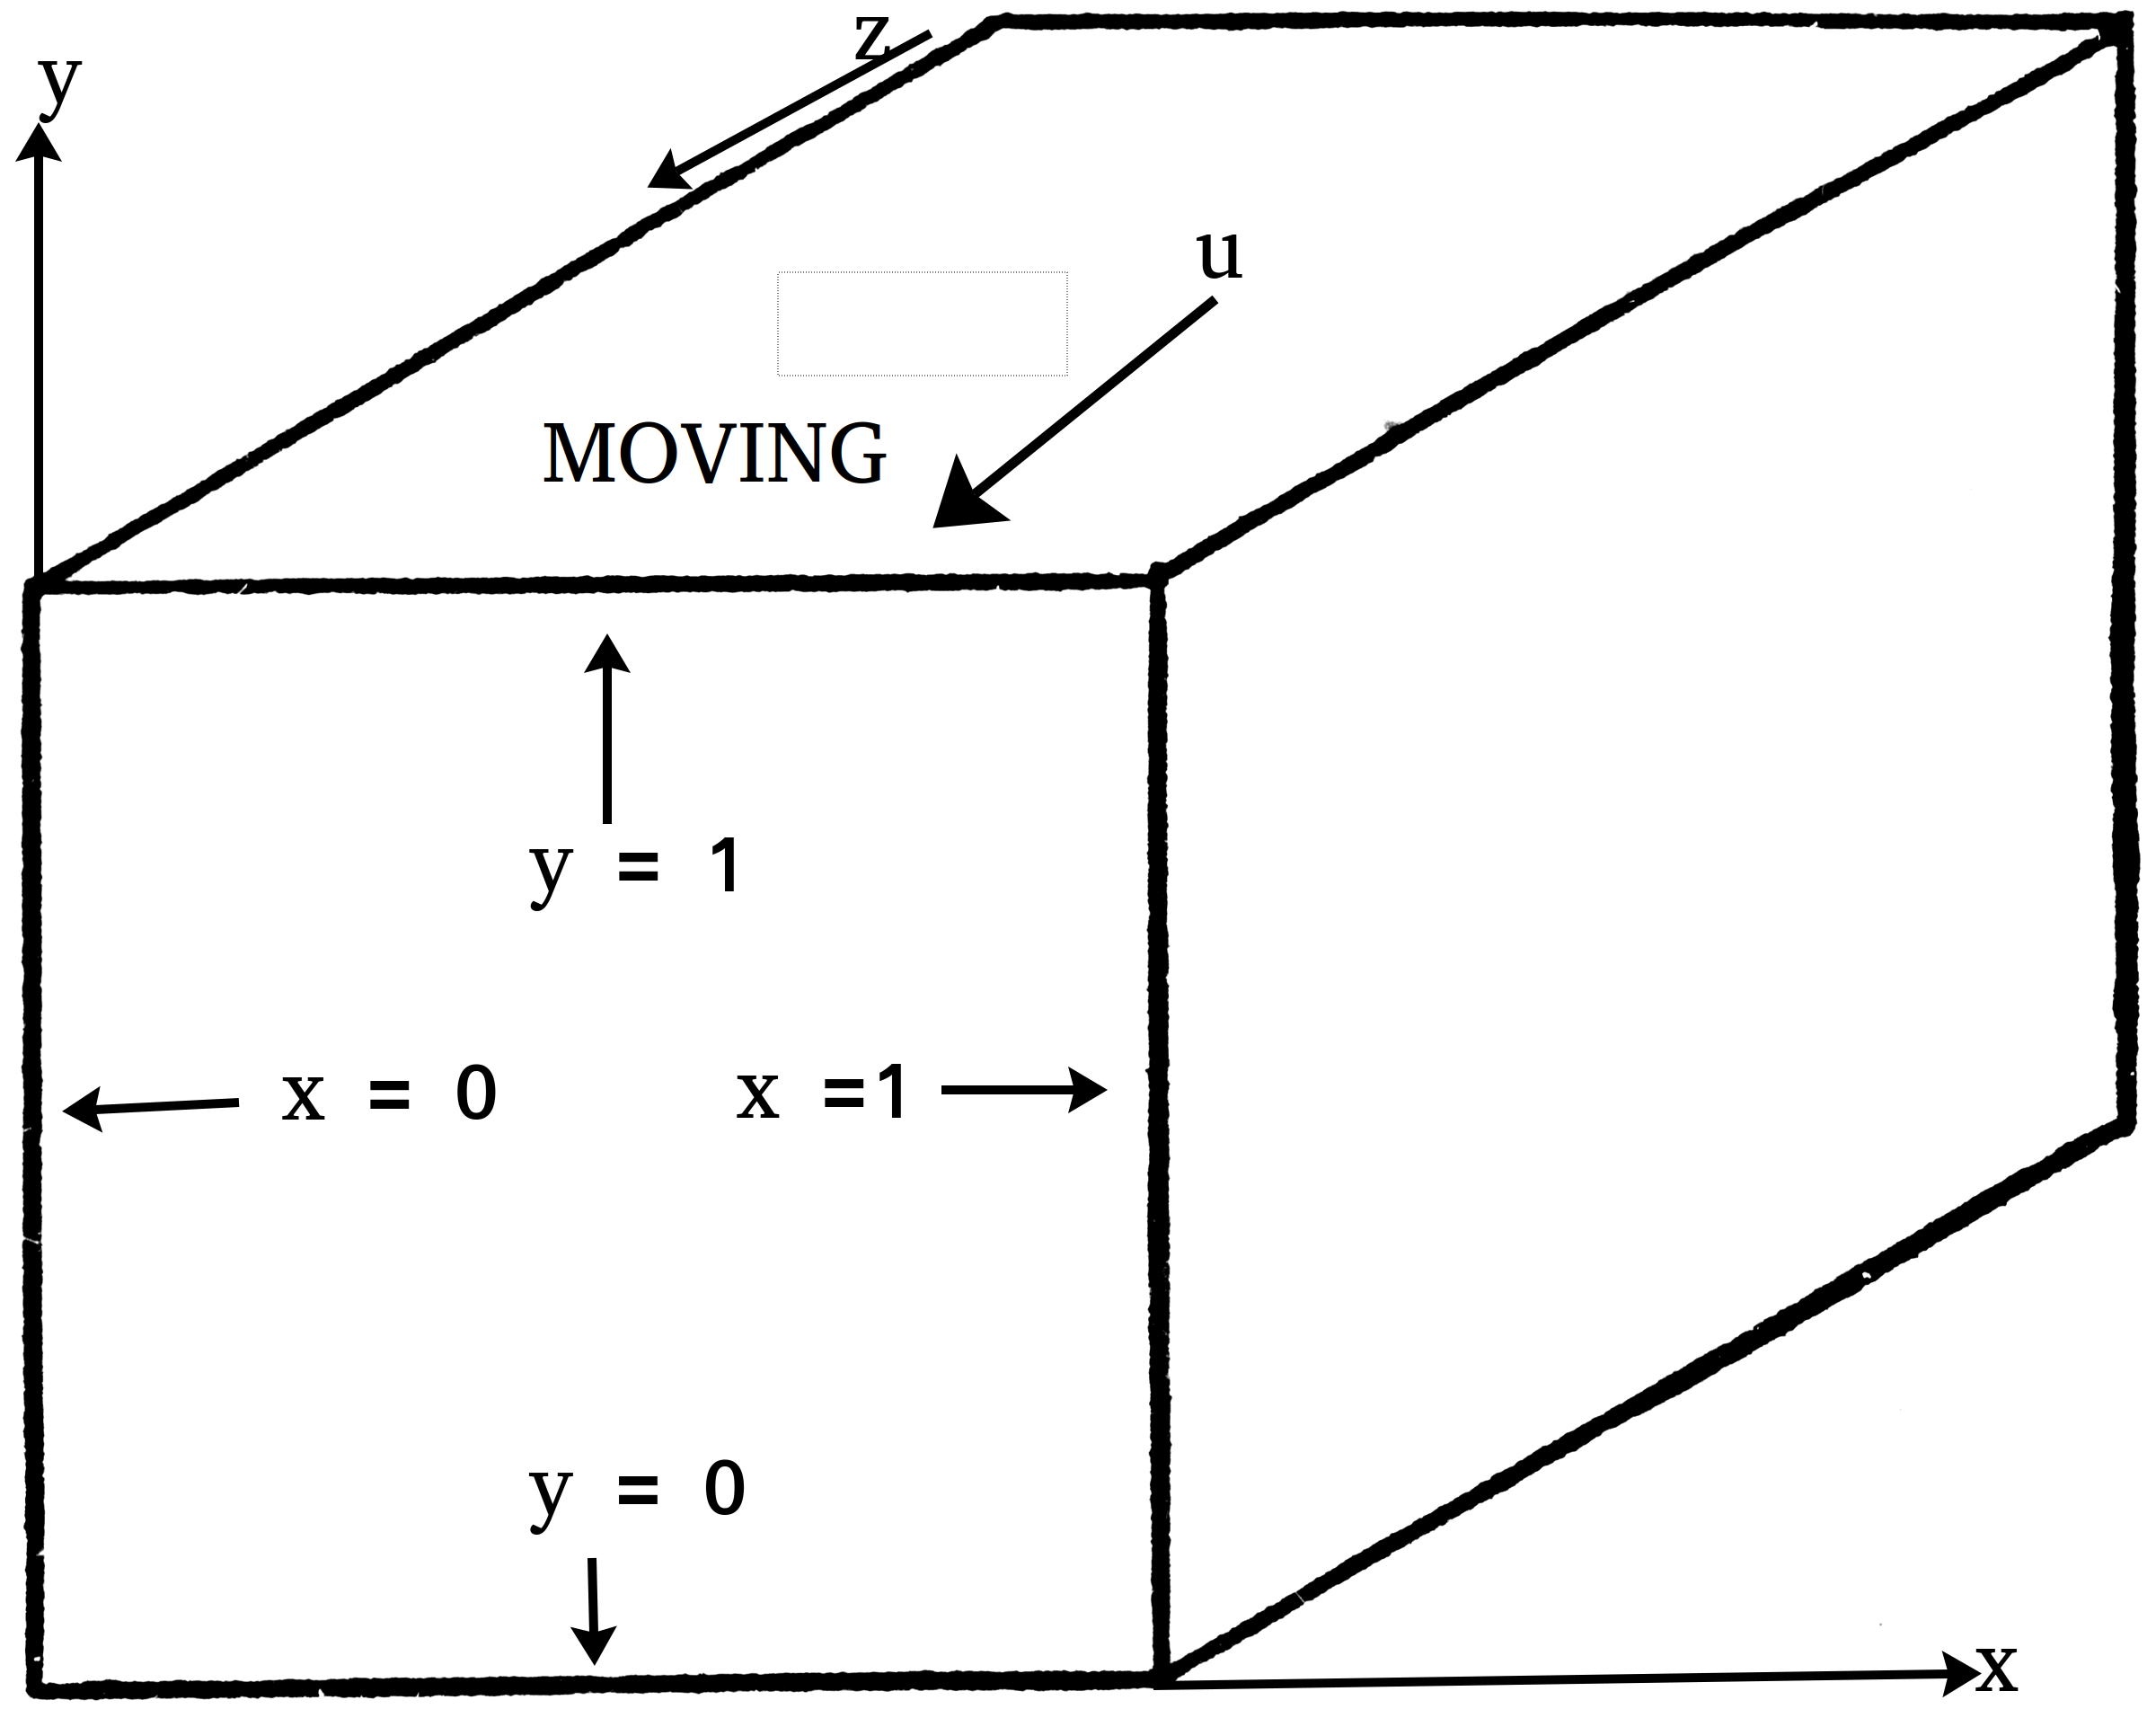
\includegraphics[width=0.6\textwidth]{/home/karl/doc/subj/att/fys4150/project5/resultsKeep/5e/boxDrawing2-0.png}
	\caption{2D problem sketch}
	\label{1}
\end{figure}

With our choise of coordinate system, positive flow represents flow out of the paper. \\

We choose $u(x,y=1) = 1$, and $u(x=0, y) = u(x=1,y) = u(x,y=0) = 0$. \\

We model the flow with the heat equation. This equation can be derived from the equations of incompressible flow, the Navier-Stokes equations, by assuming laminar flow and a flow profile of type $u = u(x,y)$:

\begin{subequations}
	\begin{align}
		\mathbf{u}_t + (\mathbf{u} \cdot \nabla) \mathbf{u} &= -\frac{\nabla p}{\rho} + \nabla^2 \mathbf{u}\\
		w(x,y)_t + (w \frac{\partial}{\partial z}) w(x,y) &\stackrel{\text{Zero pressure gradient}}{=} (\frac{\partial^2}{\partial x^2} + \frac{\partial^2}{\partial x^2} ) w(x,y)\\
		w(x,y)_t &= (\frac{\partial^2}{\partial x^2} + \frac{\partial^2}{\partial x^2} )w(x,y)\label{eq:ns}
	\end{align}
\end{subequations}

Central assumptions behind the resulting heat equation is that there is no external pressure gradient and that the flow is laminar. With turbulent flow we would have flow in all directions. This implies that our heat equation is only valid for Reynolds numbers giving laminar flow.


\begin{thebibliography}{9}
	\bibitem{MHJ} 
	Hjorth-Jensen, M.(2015)
	Computational physics. Lectures fall 2015. 
	\url{https://github.com/CompPhysics/ComputationalPhysics/tree/master/doc/Lectures}
	
	\bibitem{MHJ2}
	\url{https://github.com/CompPhysics/ComputationalPhysics/tree/master/doc/pub/pde}
	
	\bibitem{olver} 
	Olver, P.J and Shakiban, C.(2006)
	Applied linear algebra. Pearson Prentice Hall. 

\end{thebibliography}



\end{document}
